\documentclass{article}
\usepackage{graphicx} % Required for inserting images
\usepackage{amsmath}
\usepackage{enumitem}
\usepackage[paper=a4paper, margin=3cm]{geometry}
\usepackage{eurosym}
\usepackage{xcolor}
\usepackage{float}
\usepackage{pgfplots}
\usepackage[plain, onelanguage]{algorithm2e}

\title{Algorithmic Methods for Mathematical Models\\
  Course Project }
\author{Tim Wichelmann\\ \texttt{tim.wichelmann@estudiantat.upc.edu}\\[1ex] % [1ex] adds vertical space
  Jakob Eberhardt\\ \texttt{jakob.eberhardt@estudiantat.upc.edu}}
\date{\today}
\pgfplotsset{compat=1.18} 
\begin{document}

\maketitle
\thispagestyle{empty}
\newpage
\setcounter{page}{1}
\tableofcontents
% \lstlistoflistings
\listoffigures
\newpage

\section{Introduction}
In this course project, we examine and optimize the order selection and scheduling of a bakery. To this end, we formalised a model and employed CPLEX to solve the resulting Linear Integer Program~(ILP). Although it delivers an optimal solution, obtaining the order selection in this manner can take a long time for large instances. Therefore, we developed a greedy constructive algorithm that delivers a feasible and sufficient selection many orders of magnitude faster. The report includes our iterative process of further closing the optimality gap by developing and benchmarking more sophisticated greedy cost functions, employing local search, and by implementing the GRASP meta-heuristic. Finally, we summarise the achieved results. 

\section{Formal Problem Statement}
In this section, we summarise the given problem and its respective input data, the output as well as the objective.  
\subsection*{Given}
\begin{itemize}
    \item $n$ : The number of orders.
    \item $t$ : The latest time slot we consider.
    \item $profit_i$, ($1\leq i \leq n$) : Profit associated with order $i$ in \euro{}.
    \item $length_i$, ($1\leq i \leq n$) : Required number of time slots to process order $i$.
    \item $min\_deliver_i$, ($1\leq i \leq n$) : First time slot in which order $i$ can be picked up by the customer.
    \item $max\_deliver_i$, ($1\leq i \leq n$) : Last time slot order $i$ can be picked up by the customer.
    \item $surface_i$, ($1\leq i \leq n$) : Oven surface required to bake order $i$ in $m^2$.
    \item $surface\_capacity$ : Oven surface available in the bakery in $m^2$.
\end{itemize}
If an order is processed, it has to be picked up in the same time slot in which it will be finished.
Due to the limited surface capacity, the oven surface occupied by the scheduled orders can never exceed $surface\_capacity$ for any given time slot. 
At any time, the total surface of the bread that is being baked cannot exceed this capacity.
An order $i$ has to be picked up in the time range given its $min\_deliver_i$ and $max\_deliver_i$ times, including the boundaries.
% \subsection*{Auxiliary Indices} %% sind meiner Ansicht nach auch ganz normal Teil des Inputs und auch nicht wirklich Indizes -> 
% \begin{itemize}
%     \item $n$ : The number of unattended orders that can be picked for the next period.
%     \item $t$ : The number of available time slots in the next period.
% \end{itemize}

\subsection*{Output}
The output consists of a matrix of size $n \times t$.
It represents a timetable indicating if and when an order should be processed (see figure \ref{fig:extended_schedule_opt}). 

\subsection*{Objective}
Maximize the total profit, calculated as the sum of profits of each order that is successfully scheduled for the next period.

\newpage
\section{Integer Linear Programming Model}
This section includes a description of our Linear Integer Program.
\subsection{Decision variables}
\begin{itemize}
    \item $y$ is a matrix of size $n \times t$ consisting of binary variables which indicates if the order $i$ will be baked in time slot $j$.
\end{itemize}

\subsection{Auxiliary variables}

\begin{itemize}
\item $x_i$ is a binary variable indicating whether order $i$ has the right amount of time slots assigned to it. 
We use it as an indicator of whether an order is part of the schedule or not.
\item $\mathit{start}_{i}$, ($1\leq i \leq n$)denotes the time slot in which the baking process of order $i$ is started.
\item $\mathit{end}_{i}$, ($1\leq i \leq n$) denotes the time slot in which the baking process of order $i$ will be finished.
\item $\mathit{geq\_start}$ is an $n \times t$ matrix of binary variables where $\mathit{geq\_start}_{ij}$ is $1$ iff. $j$ is greater or equal to the first time slot of order $i$.
\item $\mathit{leq\_end}$ is an $n \times t$ matrix of binary variables where $\mathit{leq\_end}_{ij}$ is $1$ iff. $j$ is less or equal to the last time slot of order $i$.
\item $\mathit{min\_start}_i$, ($1\leq i \leq n$), which is the earliest possible time slot for order $i$.
    This can be done independently of other variables: 
    $$\mathit{min\_start}_i = \mathit{min\_deliver} - \mathit{length}_i + 1$$
\item $\mathit{max\_start}_i$, ($1\leq i \leq n$), which denotes the latest possible time slot for order $i$, given by
    $$\mathit{max\_start}_i=\mathit{max\_deliver} - \mathit{length}_i + 1 $$
\end{itemize}

\subsection{Objective function}

We want to maximize the total profit obtained from the selected orders

\begin{equation*}
  \max \sum^n_{i = 1} \mathit{profit}_i \: x_i.
\end{equation*}

\subsection{Constraints}

However, a possible solution is subject to the following constraints:

\begin{itemize}
 %    \item Every processed order has finished baking before the maximum delivery time: 
 %    \begin{equation}
 %    \mathit{start}_{ij}(j + \mathit{length}_i - 1) \leq \mathit{max\_deliver}_i, (1 \leq i \leq n, 1 \leq j \leq t)
 %    \end{equation}
 %    \item Every processed order has finished baking after the minimum delivery time:
 %    \begin{equation}
 %        j + \mathit{length}_i - 1 \geq \mathit{start}_{ij} \: \mathit{min\_deliver}_i, (1 \leq i \leq n, 1 \leq j \leq t) 
 %    \end{equation}
    \item In every time slot, the space capacity is respected:
    
    \begin{align}
        \sum^n_{i=1}\mathit{surface}_i \: y_{ij} &\leq \mathit{surface\_capacity}, &&(1 \leq j \leq t)
    \end{align}
    
 %    % \item The auxiliary variable $\mathit{start}_i$ has the intended meaning:
 %    % \begin{equation}
 %    %     \mathit{start}_i \leq \mathit{max\_deliver}_i - \mathit{length}_i
 %    % \end{equation}
    % \item We assign the correct amount of time slots or zero time slots to every order:
    % \begin{equation}
    %     \sum^t_{j = 1} y_{ij} = x_i \: \mathit{length}_i, (1 \leq i \leq n)
    % \end{equation}
 %    \item The time slots assigned to this order are contiguous (If an order $i$ starts in time slot $j$, it occupies the consecutive time slots from $j$ to $j + length_i$:
 % %%   \begin{equation}
 % %%       \mathit{start}_{ij} = 1 \doublearrow \sum^{j+\mathit{length}_i-1}_{k=j} y_{i,k} = \mathit{length}_i 
 % %%   \end{equation}
 %        \begin{equation}
 %        \sum^{j+\mathit{length}_i-1}_{k=j} y_{i,k} \geq \mathit{start}_{ij} \mathit{length}_i, (1 \leq i \leq n, 1 \leq j \leq t - \mathit{length}_i + 1 )
 %    \end{equation}
 %    \item Each order only has one start point:
 %    \begin{equation}
 %    \sum^{t}_{j = 1} \mathit{start}_{ij} = x_i, (1 \leq i \leq n)
 %    \end{equation}

    \item Each order is started in a time slot that allows it to finish in the delivery window:
    \begin{align}
    \mathit{start}_i &\leq \mathit{max\_start}_i, \\
    \mathit{min\_start}_i &\leq \mathit{start}_i, &&(1 \leq i \leq n)	
    \end{align}
    
    \item If an order $i$ is part of the schedule, it is assigned the $\mathit{length}_i - 1$ contiguous time slots from $\mathit{start}_i$ to $\mathit{end}_i$:
    \begin{align}
      j &\geq \mathit{start}_i - (t+1) * (1-\mathit{geq\_start}_{ij}) \\
      \mathit{start}_i &\geq j - (t+1) * \mathit{geq\_start}_{ij} \\
      \mathit{end}_i &\geq j - (t+1) * (1-\mathit{leq\_end}_{ij}) \\
      j &\geq \mathit{end}_i - (t+1) * \mathit{leq\_end}_{ij} \\
      0 &\leq \mathit{geq\_start}_{ij} + \mathit{leq\_end}_{ij} - 2 * y_{ij}, &&(1 \leq i \leq n, \mathit{min\_start}_i \leq j \leq \mathit{max\_deliver}_i) 
   \end{align}

    \item If an order $i$ is part of the schedule, its end time $\mathit{end}_i$ is equal to $\mathit{start}_i + \mathit{length}_i - 1$. 
      If order $i$ is not part of the schedule, this is indicated by the fact that $\mathit{start}_i > \mathit{end}_i$.
    \begin{align}
        \mathit{end}_i &= \mathit{start}_i + x_i \: \mathit{length}_i - 1, &&(1 \leq i \leq n)
    \end{align}

     \item %The following constraints are not necessary to obtain a correct solution.
     % But they improve the performance of the solver by eliminating infeasible solutions early on.
     % The first of these constraints is: 
     If an order is part of the schedule, we assign the correct amount of time slots to it.
     Otherwise, we assign zero time slots to it:    
    \begin{align}
        \sum^{\mathit{max\_deliver}_i}_{j = \mathit{min\_start}_i} y_{ij} &= x_i \: \mathit{length}_i, &&(1 \leq i \leq n)
    \end{align}
    
    \item There are no orders assigned to time slots that are infeasible for this order because of the delivery window:    
    \begin{align}
        \sum_{j = 1}^{\mathit{min\_start}_i-1} y_{ij} &= 0, &&(1 \leq i \leq n) \\
        \sum_{j = \mathit{max\_deliver}_i+1}^t y_{ij} &= 0, &&(1 \leq i \leq n) 
    \end{align}
\end{itemize}

\section{Greedy Algorithm and Meta-Heuristics}
In this section we describe and reason about the development of our greedy algorithm. This includes a straight-forward approach as a baseline which we continuously improve toward a 
a reliably sufficient solution compared to the optimal solution. Later, we apply local search and GRASP and tune the $\alpha$ parameter.
\subsection{Greedy constructive algorithm}\label{it:greedy_cost}
\begin{center}
\begin{algorithm}[H]
\KwIn{orders}
solution $\gets \emptyset$ \\
sortedOrders $\gets$ sort(orders, $\lambda \: x$ : orderRating($x$), DESC) \\
\ForEach{order in sortedOrders}{
    candidateSlots $\gets$ findFeasibleAssignments(order, solution)\\
    \If{$|candidateSlots| = 0$} {continue with next iteration}
    sortedCandidates $\gets$ sort(candidateSlots, $\lambda \: x$ : assignmentRating($x$, solution), DESC) \\
    candidate $\gets$ sortedCandidates[0]\\
    assign(order, startTime(candidate), solution)\\
}
\Return{solution}\;
\end{algorithm}
\end{center}

Our \textit{greedy cost function} is split into two separate calculations, one for the orders and one for the time slots.
We developed different rating criteria which are further described in section \ref{sec:comp}. We found the following combination to consistently produce good results:
\begin{itemize}
    \item For an order $i$, a function weighing its positive and negative qualities against each other:
        \begin{center}
            $$\mathit{orderRating}(i) = \frac{\mathit{profit}_i (\mathit{max\_deliver}_i - \mathit{min\_deliver}_i)}{(\mathit{length}_i \cdot \mathit{surface}_i)}$$
        \end{center} 
    \item For a possible starting time slot $j$ (for a fixed order $i$), the average percentage of space used during the baking
        \begin{center}
            $$\mathit{assignmentRating}(i,j) = \frac{\sum_{l=j}^{j + \mathit{length}_i} (\sum_{k=1}^n y_{kj} \mathit{surface}_k / \mathit{surface\_capacity})}{\mathit{length}_i}$$
        \end{center}
\end{itemize}


\subsection{Local search}

Next, we present the local search procedure which uses the \textit{first improvement} strategy to improve a solution towards a local optimum.

\begin{center}
\begin{algorithm}[H]
    \KwIn{Solution S} 
    iteration $\gets$ 0\\
    \While{time $<$ maxTime}{
        oldOrders $\gets$ sort(attendedOrders(S), $\lambda \: x$ : reassignmentRating(x), DESC)\\
        oldOrder $\gets$ oldOrders[mod(iteration, length(oldOrders))]\\
        
        currentProfit $\gets$ fitness(S)\\

        newOrders $\gets$  sort(unattendedOrders(S), $\lambda \: x$ : profit(x), DESC)\\

        oldStart $\gets$ startsAt(S, oldOrderId)\\
        unassign(S, oldOrderId)\\

        \ForEach{newOrder in newOrders}{
            assignments $\gets$  findFeasibleAssignments(S, newOrder)\\
            \If{$|$assignments$| = 0$}{
                continue with next iteration\\
            }
            move $\gets$ (oldOrder, newOrder, start(assignments[0]))\\
            neighborHighestProfit $\gets$ evaluateNeighbor(S, move)\\

            \If{currentProfit $<$ neighborHighestProfit}{
                neighbor $\gets$ createNeighborSolution(solution, move)\\
                \lIf{neighbor = NULL}{continue with next iteration}
            }
        }
        \eIf{neighbor = NULL}{
            solution.assign(oldOrderId, oldStart) \\
            iteration $\gets$ iteration + 1 \\
            continue with next iteration\\
            }
            {
                neighborFitness $\gets$ getFitness(neighbor)\\
                incumbent $\gets$ neighbor \\
                incumbentFitness $\gets$ neighborFitness \\
                iteration $\gets$ 0\\
            }
            }
    \Return{incumbent}
\end{algorithm}
\end{center}
% $$\mathit{reassignmentRating}(i) = \mathit{surface}_i$$ for an order $i$
The \textit{reassignmentRating} of a given order is equal to the surface it occupies. Removing an order with a high surface frees up more space for local search to fit in previously unused orders.

Once an old order is removed, the new orders are tried in order of profit. 
This ensures that local search can quickly increase the objective function value.

\subsection{GRASP}
Due to its greedy nature, the formally described heuristic only considers a limited set of candidates, even while other paths may lead to more profit. By employing GRASP, we achieve a configurable variability in the candidate set. By picking a random candidate within a limit, we can obtain more solutions and pick the best one while still being considerably faster compared to solving the ILP. 
\begin{center}
\begin{algorithm}[H]
\textbf{GRASP constructive phase} \\
\KwIn{orders}
solution $\gets \emptyset$ \\
\ForEach{order in orders}{
candidates $\gets$ feasibleAssignments(order, solution) \\
\If{$\lvert$candidates$\rvert = 0$}{
continue with next iteration
}
%% candidate $\gets$ selectCandidate(candidates, \alpha) \\
Evaluate $q(c)$ for all $c \in$ candidates \\
$q^{\text{min}} \gets \min \{q(c) \mid c \in$ candidates$\}$ \\
$q^{\text{max}} \gets \max \{q(c) \mid c \in$ candidates$\}$ \\
$RCL_{\text{max}} \gets \{c \in C \mid q(c) \geq q^{\text{max}} - \alpha(q^{\text{max}} - q^{\text{min}})\}$ \\
Select $c \in RCL_{\text{max}}$ at random \\
solution $\gets$ solution $\cup \: \{c\}$ \\
}
\Return solution \\
\end{algorithm}
\end{center}

Here $q(i,j)$ denotes the assignment rating we have seen before in the greedy construction phase, which is the average space usage if the order $i$ were to be scheduled at time slot $j$.

\section{Parameter Tuning}
By increasing and decreasing the $\alpha$-parameter, we can tune the variability of candidates we consider. The following plot was obtained by running our GRASP implementation on the same instance for one minute while increasing the  $\alpha$-parameter, thus adding more candidates for every respective run. Compared to the deterministic greedy solver, we consistently achieve a significantly better result by also considering previously unexplored paths. As can be seen in the plot, an alpha value of 0.8 turned out to be quite efficient while a fully randomized approach probably spends too much execution time trying out bad orders and assignments.

%%% tuning 125_plot.dat, laufzeit: 5min, alpha von 0 - 1
\begin{figure}[H]
\centering
\resizebox{0.54\textwidth}{!}{%
    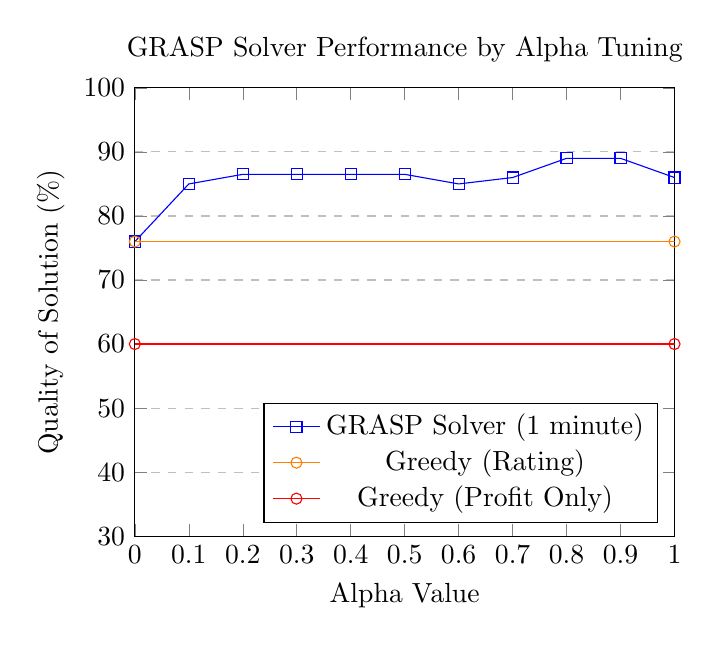
\begin{tikzpicture}
\begin{axis}[
    title={GRASP Solver Performance by Alpha Tuning},
    xlabel={Alpha Value},
    ylabel={Quality of Solution (\%)},
    xmin=0, xmax=1,
    ymin=30, ymax=100,
    xtick={0,0.1,0.2,0.3,0.4,0.5,0.6,0.7,0.8,0.9,1},
    ytick={30,40,50,60,70,80,90,100},
    legend pos=south east,
    ymajorgrids=true,
    grid style=dashed,
]

%Grasp, max obj = 146, 164, cplex
\addplot[color=blue, mark=square] coordinates {
    (0, 76) 
    (0.1, 85) % 140, 153 it
    (0.2, 86.5) % 141, 161 it
    (0.3, 86.5) % 142, 146 it 
    (0.4, 86.5) % 142 142 it
    (0.5, 86.5) % 140 157 it
    (0.6, 85) % 140 147 it
    (0.7, 86) % 141 160 it
    (0.8, 89) % 142 161 it
    (0.9, 89) % 146 150 it
    (1, 86)   % 141 149
};
\addlegendentry{GRASP Solver (1 minute)}

% Baseline solution (greedy), 126
\addplot[color=orange, mark=o] coordinates {
    (0, 76) 
    (1, 76)
};
\addlegendentry{Greedy (Rating)}
% Baseline solution (greed, profit onlyy), 97
\addplot[color=red, mark=o] coordinates {
    (0, 60) 
    (1, 60)
};
\addlegendentry{Greedy (Profit Only)}

\end{axis}
\end{tikzpicture}
}
\caption[Parameter Tuning]{This plot compares the quality of solutions when tuning the $\alpha$-parameter compared to the optimal solution and the one obtained using the Greedy solver. Each run was granted a maximum period of one minute.}
\label{fig:a_tuning}
\end{figure}

As a practical example, we computed the optimal solution of a relatively large instance of 125 pickable orders and 125 available timeslots which took more than two hours. In the following plot, we see the relative profits obtained by applying GRASP with an increasing amount of granted time compared to the optimal solution. For an alpha value of 0.8, we reach 89\% of the optimal solution within 60 seconds.
%%% Time progress grasp
\begin{figure}[H]
\centering
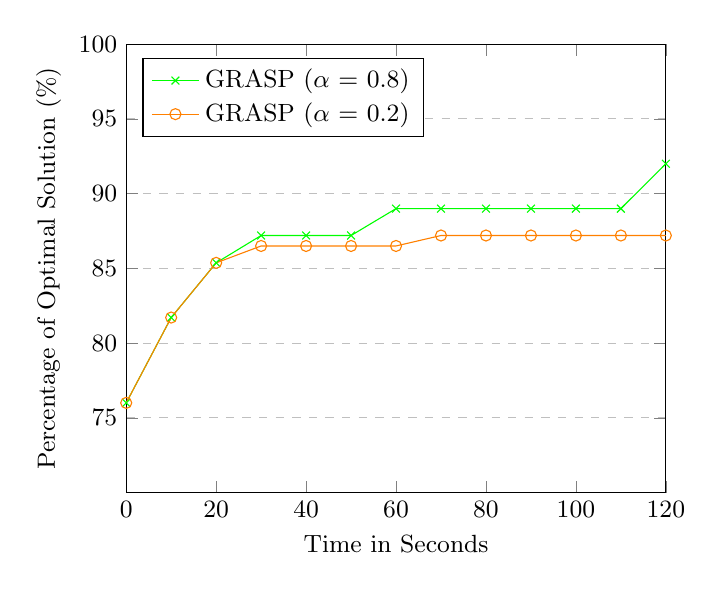
\begin{tikzpicture}
\begin{axis}[
    xlabel={Time in Seconds},
    ylabel={Percentage of Optimal Solution (\%}),
    xmin=0, xmax=120,
    ymin=70, ymax=100, % Adjusted y-axis range to fit percentage values
    xtick={0,20,40,60,80,100,120},
    ytick={75,80,85,90,95,100},
    legend pos=north west,
    ymajorgrids=true,
    grid style=dashed,
]
\addplot[color=green, mark=x] coordinates {
    (0, 76.0)
    (10, 81.71)
    (20, 85.37)
    (30, 87.20)
    (40, 87.20)
    (50, 87.20)
    (60, 89)
    (70, 89)
    (80, 89)
    (90, 89)
    (100, 89)
    (110, 89)
    (120, 92)
};
\small\addlegendentry{GRASP ($\alpha$ = 0.8)}

\addplot[color=orange, mark=o] coordinates {
    (0, 76.0)
    (10, 81.71)
    (20, 85.37)
    (30, 86.5)
    (40, 86.5)
    (50, 86.5)
    (60, 86.5)
    (70, 87.20)
    (80, 87.20)
    (90, 87.20)
    (100, 87.20)
    (110, 87.20)
    (120, 87.20)
};
\small\addlegendentry{GRASP ($\alpha$ = 0.2)}
\end{axis}
\end{tikzpicture}

\caption[Performance of GRASP as a function of time]{At $\alpha$ = 0.8, 60 seconds are usually enough to almost reach 90\% of the optimal profit.}
\label{fig:time_grasp}
\end{figure}

\section{Comparison}\label{sec:comp}
In this section, we compare the results of the previously described implementations and visualise the obtained order selections and schedules. To present the effects of our optimizations, we created solutions for the previously described instance of 125 pickable orders and 125 available timeslots using different implementations. 
In the following figure, we see an example of an optimal solution that consists of 24 picked orders which would achieve a profit of 164~\euro{}. Although it is an optimal schedule, computing it took over two hours in our local development environment.
%%% Optimal 125, 125_plot.dat, laufzeit: 3h
\begin{figure}[H]
\centering
%%% Optimal 125, 125_plot.dat, laufzeit: 3h
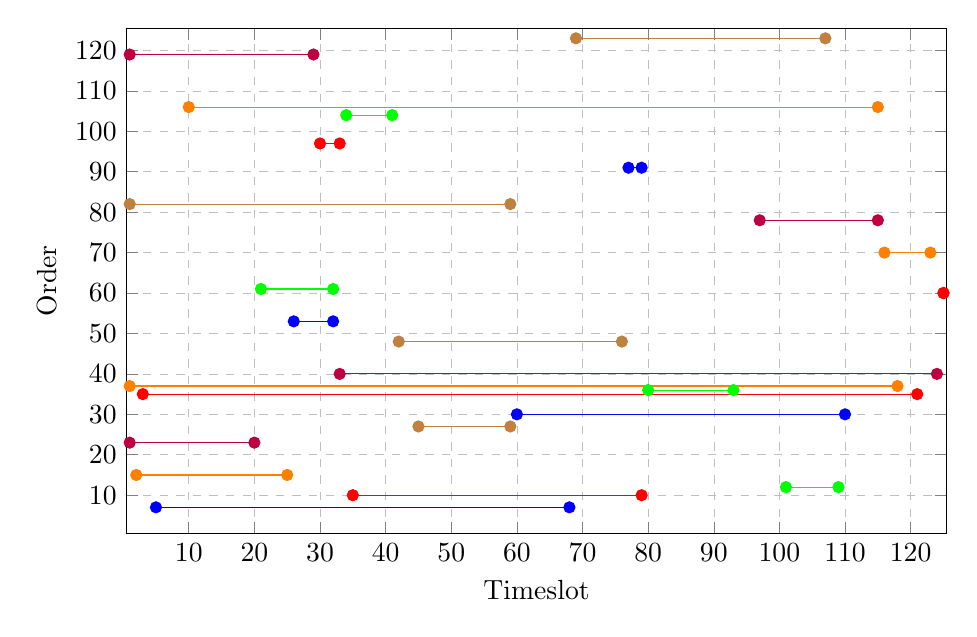
\begin{tikzpicture}
\begin{axis}[
   % title={Optimal Schedule},
    xlabel={Timeslot},
    ylabel={Order},
    xmin=0.5, xmax=125.5, 
    ymin=0.5, ymax=125.5, 
    xtick={10,20,30,40,50,60,70,80,90,100, 110, 120},
    ytick={10,20,30,40,50,60,70,80,90,100, 110, 120},
    grid=both,
    grid style={line width=.1pt, draw=gray!10},
    major grid style={line width=.2pt, draw=gray!50},
    legend pos=north east,
    ymajorgrids=true,
    xmajorgrids=true,
    grid style=dashed,
    width=12cm,
    height=8cm,
]
\addplot[color=blue, mark=*] coordinates {(5, 7) (68, 7)};
\addplot[color=red, mark=*] coordinates {(35, 10) (79, 10)};
\addplot[color=green, mark=*] coordinates {(101, 12) (109, 12)};
\addplot[color=orange, mark=*] coordinates {(2, 15) (25, 15)};
\addplot[color=purple, mark=*] coordinates {(1, 23) (20, 23)};
\addplot[color=brown, mark=*] coordinates {(45, 27) (59, 27)};
\addplot[color=blue, mark=*] coordinates {(60, 30) (110, 30)};
\addplot[color=red, mark=*] coordinates {(3, 35) (121, 35)};
\addplot[color=green, mark=*] coordinates {(80, 36) (93, 36)};
\addplot[color=orange, mark=*] coordinates {(1, 37) (118, 37)};
\addplot[color=purple, mark=*] coordinates {(33, 40) (124, 40)};
\addplot[color=brown, mark=*] coordinates {(42, 48) (76, 48)};
\addplot[color=blue, mark=*] coordinates {(26, 53) (32, 53)};
\addplot[color=red, mark=*] coordinates {(125, 60) (125, 60)};
\addplot[color=green, mark=*] coordinates {(21, 61) (32, 61)};
\addplot[color=orange, mark=*] coordinates {(116, 70) (123, 70)};
\addplot[color=purple, mark=*] coordinates {(97, 78) (115, 78)};
\addplot[color=brown, mark=*] coordinates {(1, 82) (59, 82)};
\addplot[color=blue, mark=*] coordinates {(77, 91) (79, 91)};
\addplot[color=red, mark=*] coordinates {(30, 97) (33, 97)};
\addplot[color=green, mark=*] coordinates {(34, 104) (41, 104)};
\addplot[color=orange, mark=*] coordinates {(10, 106) (115, 106)};
\addplot[color=purple, mark=*] coordinates {(1, 119) (29, 119)};
\addplot[color=brown, mark=*] coordinates {(69, 123) (107, 123)};

\end{axis}
\end{tikzpicture}
\caption[Example of an Optimal Schedule]{This schedule represents an optimal solution for a given data set of 125 orders and 125 time slots. The profit of this optimal solution is 164 \euro{}.}
\label{fig:extended_schedule_opt}
\end{figure}
The next schedule was created using the Greedy solver with a cost function tuned to only consider the profit of an order. In this case, we would only pick 13 orders which will result in a total profit of 97 \euro{}. We can account a significant portion of the optimality gap to high-profit orders which may occupy a lot of surface for a long amount of time. For example, order 14 (orange) adds 10 \euro to our total profit, yet it needs to be processed for 114 time slots while requiring 2 $m^2$ of our total capacity of 15 $m^2$. Although its individual profit is high (in this instance the highest possible profit), the order blocks the surface capacity for too long.
%%% 125 Heuristik, 125_plot.dat, getAddedValue : profit only
\begin{figure}[H]
\centering
%%% Greedy 97, 125_plot.dat, profit only
%%% E.g. order 14. altough it has a profit of 10 which is above average, it takes 114 timelots and occupies 3 slots for the basically the whole schedule. Altough they have a bit less profit, there are many orders which only take 3 surface and are way shorter to process 
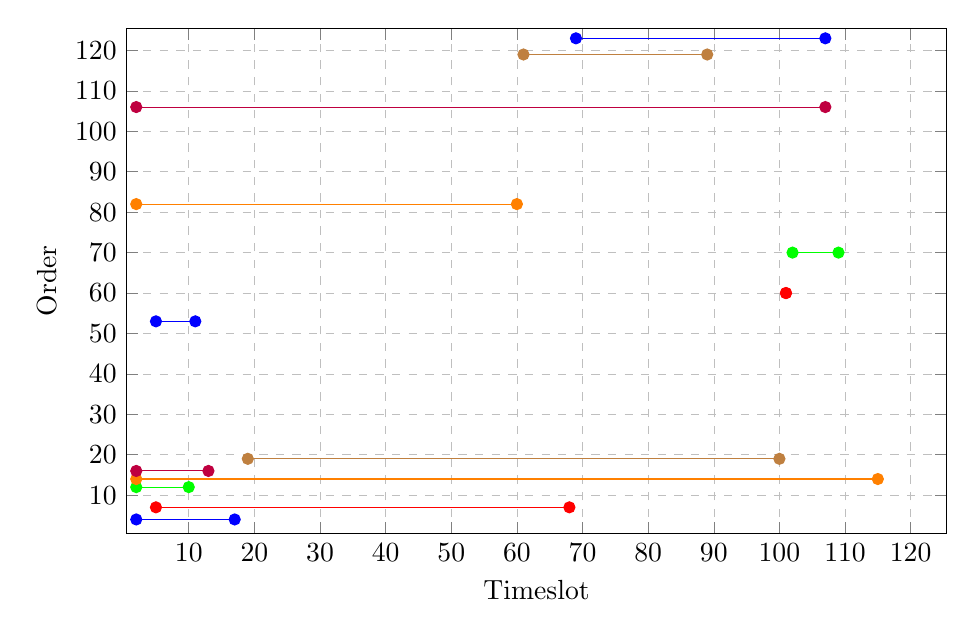
\begin{tikzpicture}
\begin{axis}[
    xlabel={Timeslot},
    ylabel={Order},
    xmin=0.5, xmax=125.5, 
    ymin=0.5, ymax=125.5, 
    xtick={10,20,30,40,50,60,70,80,90,100, 110, 120},
    ytick={10,20,30,40,50,60,70,80,90,100, 110, 120},
    grid=both,
    grid style={line width=.1pt, draw=gray!10},
    major grid style={line width=.2pt, draw=gray!50},
    legend pos=north east,
    ymajorgrids=true,
    xmajorgrids=true,
    grid style=dashed,
     width=12cm,
     height=8cm,
]
\addplot[color=blue, mark=*] coordinates {(2, 4) (17, 4)};
\addplot[color=red, mark=*] coordinates {(5, 7) (68, 7)};
\addplot[color=green, mark=*] coordinates {(2, 12) (10, 12)};
\addplot[color=orange, mark=*] coordinates {(2, 14) (115, 14)};
\addplot[color=purple, mark=*] coordinates {(2, 16) (13, 16)};
\addplot[color=brown, mark=*] coordinates {(19, 19) (100, 19)};
\addplot[color=blue, mark=*] coordinates {(5, 53) (11, 53)};
\addplot[color=red, mark=*] coordinates {(101, 60) (101, 60)};
\addplot[color=green, mark=*] coordinates {(102, 70) (109, 70)};
\addplot[color=orange, mark=*] coordinates {(2, 82) (60, 82)};
\addplot[color=purple, mark=*] coordinates {(2, 106) (107, 106)};
\addplot[color=brown, mark=*] coordinates {(61, 119) (89, 119)};
\addplot[color=blue, mark=*] coordinates {(69, 123) (107, 123)};
\end{axis}
\end{tikzpicture}
\caption[Example of an Approximated Schedule using Greedy]{This schedule was created for 125 possible orders, resulting in an optimized profit of 97 \euro{}. The greedy algorithm was tuned towards preferring orders with high profit.}
\label{fig:125_profit_approx}
\end{figure}

This schedule was created using the refined greedy cost function seen in section \ref{it:greedy_cost}. Besides the profit, we now also take the required surface and time of an order into account. Additionally, we value flexible orders with large delivery time windows. As a result, we scheduled 20 orders which led to a significantly improved profit of 126 \euro{} leaving an optimality gap of 23,2\%. If we compare it to the previous schedule, we see how order 14 left the schedule in favor of multiple smaller orders which accumulate more profit than order 14 alone. Generally, we can say that this approach works much better for the majority of instances.
%%% 125 Heuristik, 125_plot.dat, getAddedValue : Rating (see .tex file)
\begin{figure}[H]
\centering
%%% Greedy 126, 125_plot.dat,         return (self.profit * (self.max_deliver - self.min_deliver)) / (self.length * self.surface)
%%% Dropped order 14 in favor of many small orders
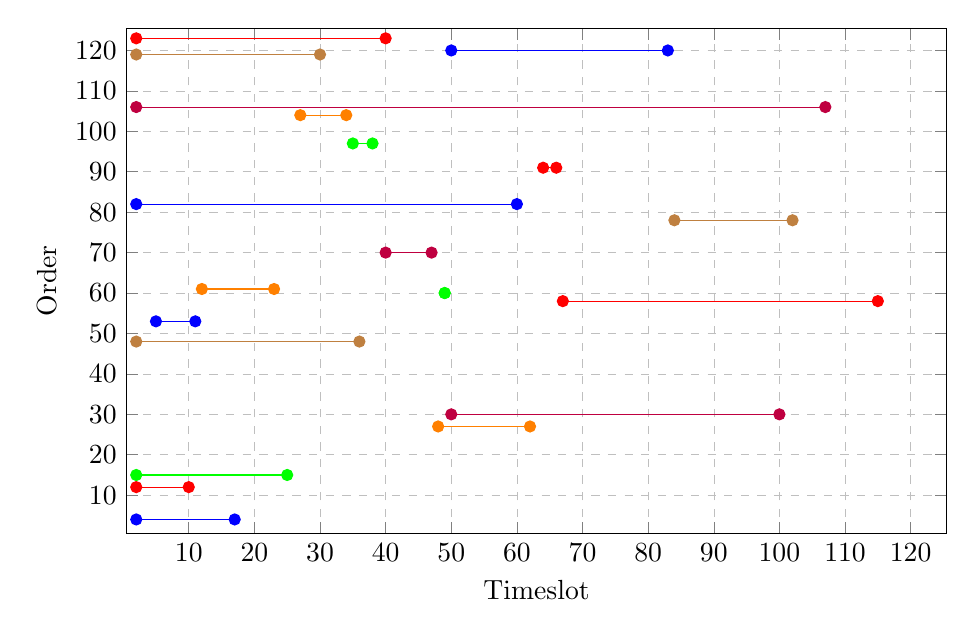
\begin{tikzpicture}
\begin{axis}[
    xlabel={Timeslot},
    ylabel={Order},
    xmin=0.5, xmax=125.5, 
    ymin=0.5, ymax=125.5, 
    xtick={10,20,30,40,50,60,70,80,90,100, 110, 120},
    ytick={10,20,30,40,50,60,70,80,90,100, 110, 120},
    grid=both,
    grid style={line width=.1pt, draw=gray!10},
    major grid style={line width=.2pt, draw=gray!50},
    legend pos=north east,
    ymajorgrids=true,
    xmajorgrids=true,
    grid style=dashed,
     width=12cm,
     height=8cm,
]
\addplot[color=blue, mark=*] coordinates {(2, 4) (17, 4)};
\addplot[color=red, mark=*] coordinates {(2, 12) (10, 12)};
\addplot[color=green, mark=*] coordinates {(2, 15) (25, 15)};
\addplot[color=orange, mark=*] coordinates {(48, 27) (62, 27)};
\addplot[color=purple, mark=*] coordinates {(50, 30) (100, 30)};
\addplot[color=brown, mark=*] coordinates {(2, 48) (36, 48)};
\addplot[color=blue, mark=*] coordinates {(5, 53) (11, 53)};
\addplot[color=red, mark=*] coordinates {(67, 58) (115, 58)};
\addplot[color=green, mark=*] coordinates {(49, 60) (49, 60)};
\addplot[color=orange, mark=*] coordinates {(12, 61) (23, 61)};
\addplot[color=purple, mark=*] coordinates {(40, 70) (47, 70)};
\addplot[color=brown, mark=*] coordinates {(84, 78) (102, 78)};
\addplot[color=blue, mark=*] coordinates {(2, 82) (60, 82)};
\addplot[color=red, mark=*] coordinates {(64, 91) (66, 91)};
\addplot[color=green, mark=*] coordinates {(35, 97) (38, 97)};
\addplot[color=orange, mark=*] coordinates {(27, 104) (34, 104)};
\addplot[color=purple, mark=*] coordinates {(2, 106) (107, 106)};
\addplot[color=brown, mark=*] coordinates {(2, 119) (30, 119)};
\addplot[color=blue, mark=*] coordinates {(50, 120) (83, 120)};
\addplot[color=red, mark=*] coordinates {(2, 123) (40, 123)};
\end{axis}
\end{tikzpicture}
\caption[Example of an Approximated Schedule based on an Advanced Cost Function]{Computing this schedule took one second. It would result in an optimized profit of 126 \euro{}. The greedy algorithm was tuned towards preferring short orders with little surface requirement, but also considering the profit.}
\label{fig:125_schedule_approx}
\end{figure}


The last schedule was created by running the GRASP solver for one minute at an $\alpha$-value of 0.8. Randomizing the candidate selection to a certain extent allows us to explore a variety of paths and achieve an optimized profit of 146 \euro{} which leaves us with an optimality gap of 11\% for this given instance.
%%% 125 GRASP, 125_plot.dat, random assignments a=1, t=120
\begin{figure}[H]
\centering
%%% GRASP, a=0.8, obj= 5min, 5 iterations, 
% Profit = 146
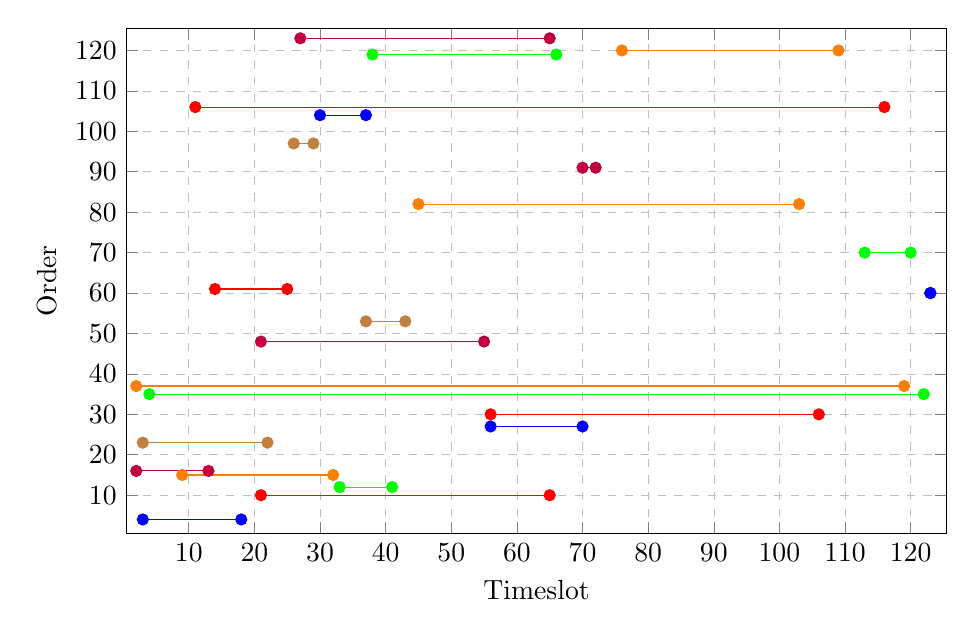
\begin{tikzpicture}
\begin{axis}[
    xlabel={Timeslot},
    ylabel={Order},
    xmin=0.5, xmax=125.5, 
    ymin=0.5, ymax=125.5, 
    xtick={10,20,30,40,50,60,70,80,90,100, 110, 120},
    ytick={10,20,30,40,50,60,70,80,90,100, 110, 120},
    grid=both,
    grid style={line width=.1pt, draw=gray!10},
    major grid style={line width=.2pt, draw=gray!50},
    legend pos=north east,
    ymajorgrids=true,
    xmajorgrids=true,
    grid style=dashed,
     width=12cm,
     height=8cm,
]
\addplot[color=blue, mark=*] coordinates {(3, 4) (18, 4)};
\addplot[color=red, mark=*] coordinates {(21, 10) (65, 10)};
\addplot[color=green, mark=*] coordinates {(33, 12) (41, 12)};
\addplot[color=orange, mark=*] coordinates {(9, 15) (32, 15)};
\addplot[color=purple, mark=*] coordinates {(2, 16) (13, 16)};
\addplot[color=brown, mark=*] coordinates {(3, 23) (22, 23)};
\addplot[color=blue, mark=*] coordinates {(56, 27) (70, 27)};
\addplot[color=red, mark=*] coordinates {(56, 30) (106, 30)};
\addplot[color=green, mark=*] coordinates {(4, 35) (122, 35)};
\addplot[color=orange, mark=*] coordinates {(2, 37) (119, 37)};
\addplot[color=purple, mark=*] coordinates {(21, 48) (55, 48)};
\addplot[color=brown, mark=*] coordinates {(37, 53) (43, 53)};
\addplot[color=blue, mark=*] coordinates {(123, 60) (123, 60)};
\addplot[color=red, mark=*] coordinates {(14, 61) (25, 61)};
\addplot[color=green, mark=*] coordinates {(113, 70) (120, 70)};
\addplot[color=orange, mark=*] coordinates {(45, 82) (103, 82)};
\addplot[color=purple, mark=*] coordinates {(70, 91) (72, 91)};
\addplot[color=brown, mark=*] coordinates {(26, 97) (29, 97)};
\addplot[color=blue, mark=*] coordinates {(30, 104) (37, 104)};
\addplot[color=red, mark=*] coordinates {(11, 106) (116, 106)};
\addplot[color=green, mark=*] coordinates {(38, 119) (66, 119)};
\addplot[color=orange, mark=*] coordinates {(76, 120) (109, 120)};
\addplot[color=purple, mark=*] coordinates {(27, 123) (65, 123)};
\end{axis}
\end{tikzpicture}
\caption[Example of an Approximated Schedule using GRASP]{By running the GRASP meta-heuristic for one minute, we get a schedule that will result in a profit of 146 \euro{}.}
\label{fig:125_schedule_approx_grasp}
\end{figure}


In the following plot, we can see that our refined greedy cost function works well for most instances. We can consistently enhance the greedy solution by additionally running local search for 30 seconds. Using GRASP, we can reliably obtain a very good solution within one minute.
%%% Size vs Quality 
\begin{figure}[H]
\centering
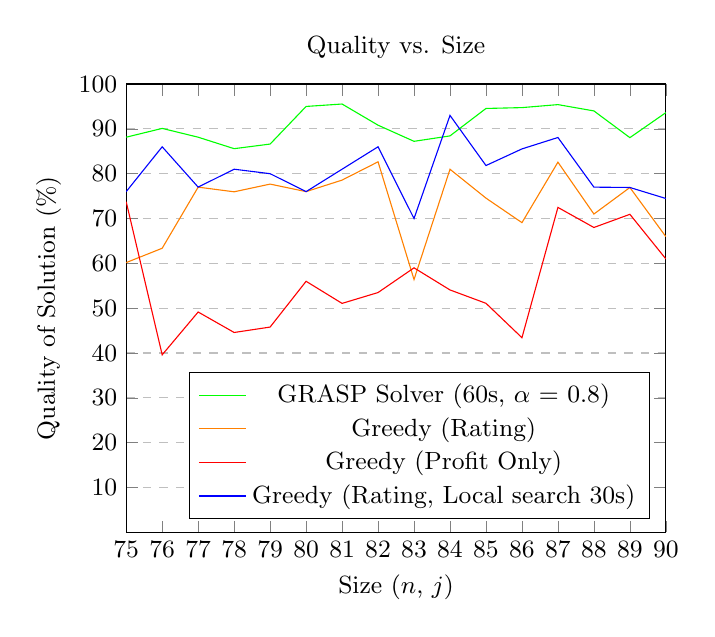
\begin{tikzpicture}
\begin{axis}[
    title={Quality vs. Size},
    xlabel={Size ($n$, $j$)},
    ylabel={Quality of Solution (\%)},
    xmin=75, xmax=90,
    ymin=0, ymax=100,
    xtick={75,76,77,78,79,80,81,82,83,84,85,86,87,88,89, 90},
    ytick={10, 20, 30, 40,50,60,70,80,90,100},
    legend pos=south east,
    ymajorgrids=true,
    grid style=dashed,
    %legend style={at={(1.05,1)},anchor=north west}
]

% GRASP Solver (1 minutes)
\addplot[color=green] coordinates {
    (75, 88.14)
    (76, 90.10)
    (77, 88.14)
    (78, 85.58)
    (79, 86.61)
    (80, 95)
    (81, 95.54)
    (82, 90.82)
    (83, 87.22)
    (84, 88.43)
    (85, 94.55)
    (86, 94.74)
    (87, 95.41)
    (88, 94)
    (89, 88.04)
    (90, 93.62)
};
\small\addlegendentry{GRASP Solver (60s, $\alpha$ = 0.8)}

% Greedy (Rating)
\addplot[color=orange] coordinates {
    (75, 60.17)
    (76, 63.37)
    (77, 77.00)
    (78, 75.96)
    (79, 77.68)
    (80, 76)
    (81, 78.57)
    (82, 82.65)
    (83, 56.39)
    (84, 80.99)
    (85, 74.55)
    (86, 69.08)
    (87, 82.57)
    (88, 71)
    (89, 76.92)
    (90, 65.96)
};
\addlegendentry{Greedy (Rating)}

% Greedy (Profit Only)
\addplot[color=red] coordinates {
    (75, 73.73)
    (76, 39.60)
    (77, 49.15)
    (78, 44.58)
    (79, 45.79)
    (80, 56)
    (81, 51.07)
    (82, 53.49)
    (83, 59.0)
    (84, 54.07)
    (85, 51.09)
    (86, 43.42)
    (87, 72.48)
    (88, 68)
    (89, 70.94)
    (90, 60.99)
};
% (75, 73.73)
%     (76, 39.60)
%     (77, 49.15)
%     (78, 35.58)
%     (79, 26.79)
%     (80, 51)
%     (81, 41.07)
%     (82, 74.49)
%     (83, 60.90)
%     (84, 52.07)
%     (85, 29.09)
%     (86, 43.42)
%     (87, 72.48)
%     (88, 68)
%     (89, 70.94)
%     (90, 60.99)
% };
\addlegendentry{Greedy (Profit Only)}

% Greedy with localsearch
\addplot[color=blue] coordinates {
    (75, 76)
    (76, 86)
    (77, 77)
    (78, 81)
    (79, 80)
    (80, 76)
    (81, 81)
    (82, 86)
    (83, 70)
    (84, 93)
    (85, 81.8181818181818)
    (86, 85.5263157894737)
    (87, 88.0733944954128)
    (88, 77)
    (89, 76.9230769230769)
    (90, 74.468085106383)
};
\addlegendentry{Greedy (Rating, Local search 30s)}


\end{axis}
\end{tikzpicture}

%%% With symbols
% % GRASP Solver (5 minutes)
% \addplot[color=blue, mark=square] coordinates {
%     (75, 88.14)
%     (76, 90.10)
%     (77, 88.14)
%     (78, 85.58)
%     (79, 86.61)
%     (80, 95)
%     (81, 95.54)
%     (82, 90.82)
%     (83, 87.22)
%     (84, 88.43)
%     (85, 94.55)
%     (86, 94.74)
%     (87, 95.41)
%     (88, 94)
%     (89, 88.04)
%     (90, 93.62)
% };
% \addlegendentry{GRASP Solver (5 minutes)}

% % Greedy (Rating)
% \addplot[color=orange, mark=o] coordinates {
%     (75, 60.17)
%     (76, 63.37)
%     (77, 77.97)
%     (78, 75.96)
%     (79, 77.68)
%     (80, 76)
%     (81, 78.57)
%     (82, 82.65)
%     (83, 56.39)
%     (84, 80.99)
%     (85, 74.55)
%     (86, 69.08)
%     (87, 82.57)
%     (88, 71)
%     (89, 76.92)
%     (90, 65.96)
% };
% \addlegendentry{Greedy (Rating)}

% % Greedy (Profit Only)
% \addplot[color=red, mark=o] coordinates {
%     (75, 73.73)
%     (76, 39.60)
%     (77, 49.15)
%     (78, 35.58)
%     (79, 26.79)
%     (80, 51)
%     (81, 41.07)
%     (82, 74.49)
%     (83, 60.90)
%     (84, 52.07)
%     (85, 29.09)
%     (86, 43.42)
%     (87, 72.48)
%     (88, 68)
%     (89, 70.94)
%     (90, 60.99)
% };
% \addlegendentry{Greedy (Profit Only)}

% % Greedy with localsearch
% \addplot[color=green, mark=square] coordinates {
%     (75, 76)
%     (76, 86)
%     (77, 77)
%     (78, 81)
%     (79, 80)
%     (80, 76)
%     (81, 81)
%     (82, 86)
%     (83, 70)
%     (84, 93)
%     (85, 81.8181818181818)
%     (86, 85.5263157894737)
%     (87, 88.0733944954128)
%     (88, 77)
%     (89, 76.9230769230769)
%     (90, 74.468085106383)
% };
% \addlegendentry{Greedy (Rating, Localsearch 45s)}
\caption[Solution Quality]{The quality of the solution obtained with different solvers compared to an optimal solution.}
\label{fig:timequality}
\end{figure}


Since we need to submit our order selection in time, an increasing instance size quickly establishes a border at which it makes no sense to compute an optimal solution. However, we can still generate a sufficiently good selection for much larger instances in a fraction of the time by using our heuristic approach. For example, with our given computing resources, we would be able to reliably compute an optimal solution in time for instances with more than 150 orders and 150 available timeslots. The greedy solver allows us to go far beyond this limit while still delivering good results, especially in combination with local search and GRASP.
%%% Greedy time 
\begin{figure}[H]
\centering
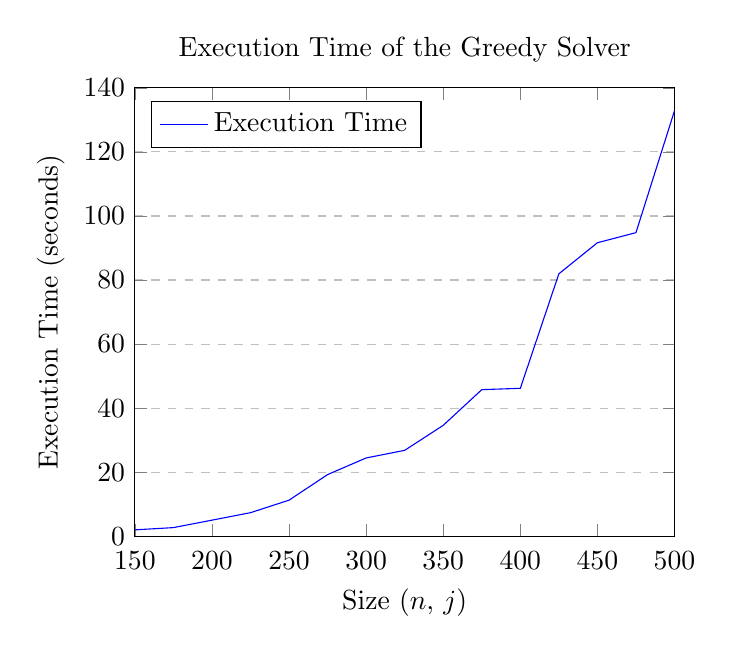
\begin{tikzpicture}
\begin{axis}[
    title={Execution Time of the Greedy Solver},
    xlabel={Size ($n$, $j$)},
    ylabel={Execution Time (seconds)},
    xmin=150, % Set minimum x value to 150
    xmax=500, % Set maximum x value
    xtick={150,200,250,300,350,400,450,500},
    xticklabels={150,200,250,300,350,400,450,500},
    ymin=0, % Set minimum y value to 0
    ymax=140, % Set maximum y value
    ytick={0,20,40,60,80,100,120,140}, % Set y ticks in steps of 20
    symbolic x coords={150,175,200,225,250,275,300,325,350,375,400,425,450,475,500},
    xticklabel style={anchor=base, yshift=-\baselineskip},
    yticklabel style={/pgf/number format/fixed},
    legend pos=north west,
    ymajorgrids=true,
    grid style=dashed,
]
\addplot[
    color=blue,
    ]
    coordinates { % 
    (150,1.98) (175,2.68) (200,5.01) (225,7.34) (250,11.25) (275,19.24) (300,24.43) (325,26.81) (350,34.62) (375,45.76) (400,46.18) (425,81.94) (450,91.64) (475,94.79) (500,132.87)
    };
    \legend{Execution Time}
\end{axis}
\end{tikzpicture}
\caption[Greedy on very big Instances]{The Greedy implementation can provide feasible and profitable schedules within very little time compared to CPLEX.}
\label{fig:grasp_time}
\end{figure}
\newpage
The time needed to compute the optimal solution is very sensitive to the instance size but also depends on the input data itself. Therefore, obtaining an optimal solution using CPLEX does not scale well, as can be seen in the following plot.
%% Size vs time cplex
\begin{figure}[H]
        \centering
        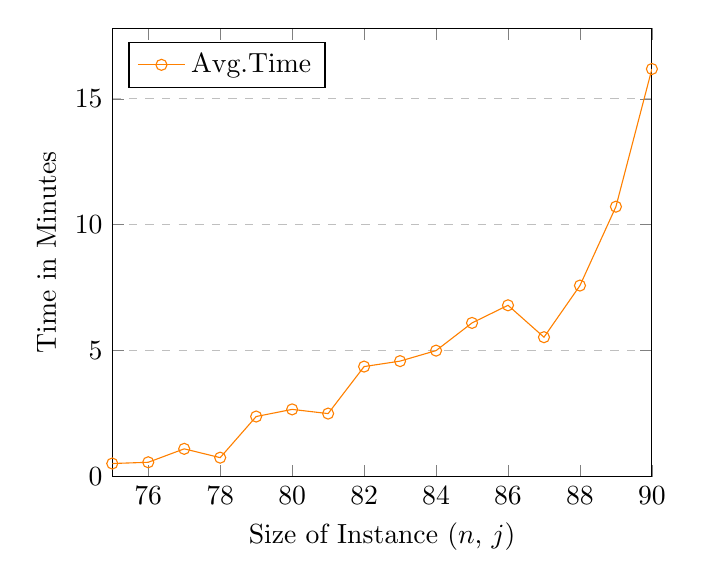
\begin{tikzpicture}
\begin{axis}[
    xlabel={Size of Instance ($n$, $j$)},
    ylabel={Time in Minutes},
    xmin=75, xmax=90,
    ymin=0, % Adjust ymin and ymax as needed
    legend pos=north west,
    ymajorgrids=true,
    grid style=dashed,
]
\addplot[color=orange, mark=o] coordinates {
    (75, 31/60)
    (76, 34/60)
    (77, 66/60)
    (78, 45/60)
    (79, 143/60)
    (80, 160/60)
    (81, 150/60)
    (82, 262/60)
    (83, 275/60)
    (84, 300/60)
    (85, 366/60)
    (86, 408/60)
    (87, 332/60)
    (88, 455/60)
    (89, 643/60)
    (90, 971/60)
};
\addlegendentry{Avg.Time}
\end{axis}
\end{tikzpicture}

        \caption[Time for solving the ILP]{Avarage time needed to obtain an optimal solution for an increasingly large instance using CPLEX.}
        \label{fig:timecplex}
\end{figure}


\section{Future Prospects}
For the greedy algorithm, there is the possibility to try different combinations of order/time slot greedy cost functions.
In the case of GRASP, we could apply the RCL to the list of sorted orders to explore more diverse solutions.

\section{Summary}

In this project, we formally modeled the problem of picking and scheduling orders to maximize the profit of the bakery and used CPLEX to find optimal solutions for generated data sets.
Since obtaining an optimal solution for a large instance can take a long time, we also developed heuristic approaches to generate feasible schedules that result in a good profit. To this end, we first implemented a greedy algorithm which is tuned towards picking high-profit orders. As described in figure \ref{fig:125_profit_approx}, this approach tends to cloak the schedule with a few profitable orders which can result in a rather high optimality gap for most instances. Hence, we developed a greedy cost function that favors flexible, small, and short orders that still add a reasonable profit (see \ref{it:greedy_cost}) which results in much better profits. Local search was used as an improvement to the greedy algorithm to include feasible high-profit orders that the greedy algorithm occasionally misses. Lastly, we applied the GRASP meta-heuristic to our greedy solver and tuned the alpha value to further close the optimallity gap towards a consistent single-digit percentage in a short amount of time. 
\end{document}
